\section[Use Cases for \acl{WIC}]{Harvest and Loading Processes as Use Cases for \acl{WIC}}
The Forage harvester has proven to be an essential agricultural machine for harvesting and loading forage. \textcite{seifert_feldhacksler_1962} define a forage harvester
as an agricultural loading machine for nearly all types of animal feed. According to the authors, a forage harvester can load the following animal feed by mounting different cutting and loading devices: Hey, Straw, Corn, Grass and Clover.
\begin{figure}%
	\centering
	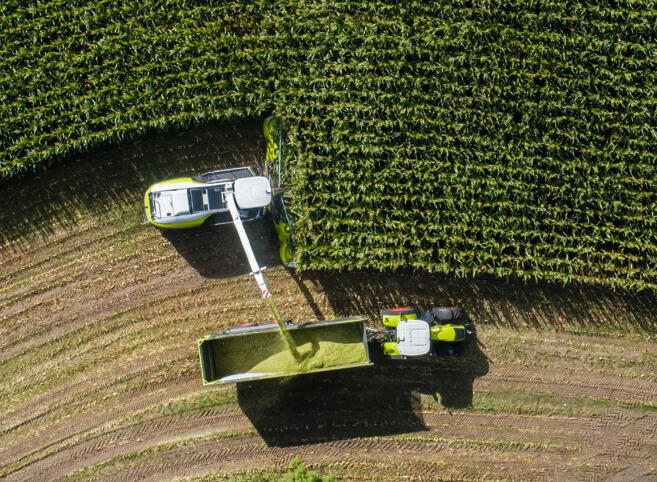
\includegraphics[width=0.6\textwidth]{figures/claas_harvest_side.png}
	\caption{\acf{FH} and \acf{TM} in a corn harvesting and loading process}%
	\label{fig:normal}%
\end{figure}

In the harvesting and loading process, a \ac{TM} typically drives alongside or behind the \ac{FH} so that the \ac{FH} can load the harvested goods onto the trailer of the \ac{TM} using the spout. Drivers operate both machines and try to keep the speed and distance so that the spout only throws the harvested goods into the trailer of the TM. An image of a corn harvesting and loading process can be seen in \autoref{fig:normal}.

Taking a corn harvest scenario as an example, some key figures are represented in \cite{faustzahlen2018}, a standard reference book in agricultural literature. This book contains key figures of agricultural processes, which 80 experts have compiled.
The key figures, which are shown in \autoref{tab:DataSilageHarvest}, are dependent on the \ac{PD} and show the large amount of forage harvested by a \ac{FH} every hour.
\begin{table}[H]
	\centering
	\begin{tabular}{>{\raggedright}p{4.9cm}p{1.8cm}p{1.8cm}p{1.8cm}}
		\toprule
  		\acf{PD}&\SI{20}{\tonne\per\hectare}&\SI{30}{\tonne\per\hectare} & \SI{50}{\tonne\per\hectare}\\
		\midrule
		Required \acl{TM}s & \num{5}&
		\num{7} & \num{10} \\
		Harvested volume in \si{\cubic\metre\per\hour} &
		\num{285.7}-\num{333.3}
		& \num{428.6}-\num{500.0} &
		\num{595.7}-\num{695.0}\\
		Filled \acl{TM} loads in \si{\per\hour} &
		\num{5.7} - \num{6.7}
		& \num{8.6} - \num{10.0} &
		\num{11.9} - \num{13.9}\\
		Harvested mass in \si{\tonne\per\hour} & \num{100}
		& \num{150} &
		\num{208.5} \\
		\bottomrule
	\end{tabular}
	\caption{Key figures of corn harvest of a \acf{FH} with a working width of \SI{6.2}{\metre} in a \SI{80}{\hectare}-field in regards to \acf{PD}  \cite{faustzahlen2018}}
	\label{tab:DataSilageHarvest}
\end{table}

The harvesting and loading processes are examples of the use of agricultural Platooning Services as described by
\textcite{zhang_method_2009}.
This Platooning Service creates a leader and follower system where an uncrewed agricultural machine follows a leading operated agricultural machine.
The operated \ac{FH}, as a leader, sets the path and speed and transmits the data via \ac{WIC} to the \ac{TM}. Based on the path and speed data of the \ac{FH}, \ac{TM} follows unmanned with a longitudinal and lateral offset, as \autoref{fig:offset} displays.
\begin{figure}[H]
	\centering
	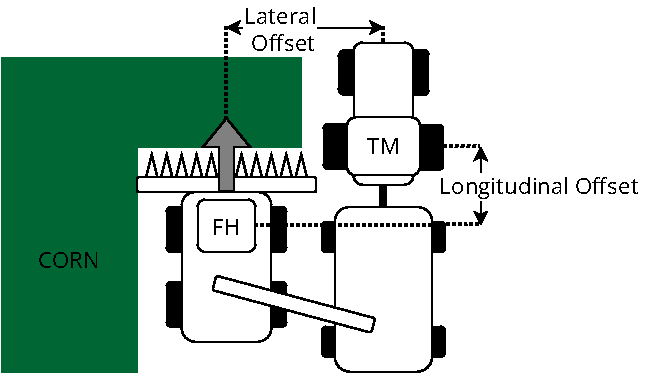
\includegraphics[width=0.65\textwidth]{figures/offset_platoon.pdf}
	\caption{Lateral and longitudinal offset between the two agricultural machines \acf{FH} and \acf{TM} in a corn harvest scenario}%
	\label{fig:offset}%
\end{figure}

The application of platooning services offers many advantages.
The \ac{TM} is positioned optimally to the \ac{FH} so that the forage can be loaded ideally from the \ac{FH} onto the \ac{TM}.

Because, as displayed in \autoref{fig:workforce_agri}, fewer and fewer workers are working in agriculture, platooning services for harvest and loading processes can save and free up labour for other activities \cite{liu_automation_2022}. As stated in \autoref{tab:DataSilageHarvest}, ten drivers for the \ac{TM}s are needed in the corn harvest process with a high \ac{PD}. Using an agricultural Platooning Service, each \ac{TM} can drive unmanned in the field, leading to fewer workers needed in the corn harvest process.

\begin{figure}[H]
	\centering
	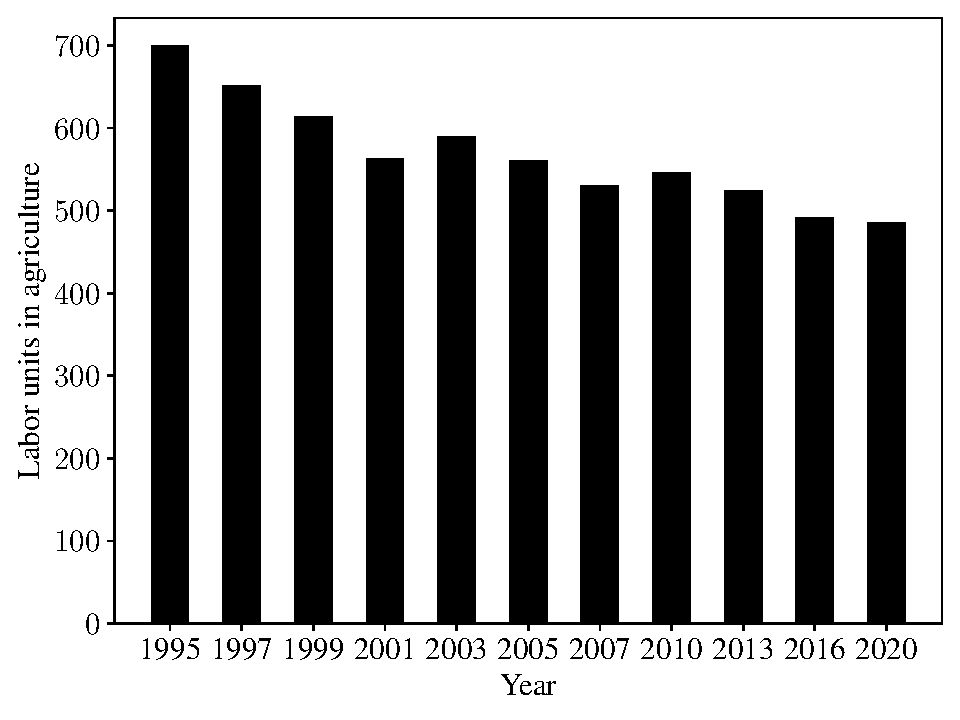
\includegraphics[width=0.75\textwidth]{figures/WorkForceAgriculture.pdf}
	\caption{Decrease in the agricultural labor force in Germany based on the data from \cite{bmel2020}}%
	\label{fig:workforce_agri}%
\end{figure}

\textcite{smolnik_5g_2020} adds that platooning services at the platoon level can reduce \ac{FH} drivers' workload so that they can focus on optimally adjusting the machines.
In addition, \ac{TM}s can be guided to the \ac{FH}s in a targeted manner so that logistics processes in the field can be improved.

At the same time, the harvest and loading processes are examples of the video streaming \ac{WIC} use case, where a video of the \ac{TM}'s filllevel is available at the \ac{FH} and could be transmitted to the \ac{TM} in order to inform the \ac{TM} driver about the machines filllevel. During these harvest and loading processes, the spout of the \ac{FH} must be controlled to set the loading position of the forage into the trailer of the \ac{TM}.

According to \textcite{murcia_quadrotor_2014}, different spout guidance and control systems have been developed to automate the filling of the trailer. Spout guidance and control systems use a camera attached to the spout to determine the fill volume at each point of the trailer via machine vision and set the spout to fill the empty parts accordingly. The author describes Autofill - systems from Claas and Intellifill - systems from CNH Industrial as examples of spout guidance systems.

Streaming the video of a camera at the spout from the \ac{FH} to the \ac{TM} would be a practical application of the video streaming use case in the harvesting process. If the \ac{TM} driver can watch a live stream of the trailer's fill level, he will always be
informed and knows when the trailer is full and can drive the forage back to the
farm.

